\part{Optimal Control and Optimal Estimation}



\chapter{LQR Design via Quadratic Programming}
\label{chap:lqr}

\begin{quote}
	\textit{``The linear variance-minimisation problem... constitutes the most complete and elegant part of optimal control theory.''} \\
	
	\hfill --- \textbf{Huibert Kwakernaak \& Raphael Sivan}, \textit{Linear Optimal Control Systems} (1972)
\end{quote}

In the preceding chapters, we focused on modelling dynamical systems and analysing their fundamental properties such as stability, controllability, and observability. We now transition from \textit{analysis} to \textit{synthesis}. How do we design a controller that not only stabilises a system but does so in the best possible way?

The Linear Quadratic Regulator (LQR) is a foundational result in optimal control theory. It provides a systematic method to trade off regulation performance against control effort. Traditionally, this problem is introduced via the algebraic Riccati equation—a recursive solution ideal for infinite-horizon unconstrained problems. However, to fully grasp Model Predictive Control (MPC), we must view LQR through a different lens.

In this chapter, we adopt a numerical optimisation perspective. Instead of solving the control problem recursively (time-step by time-step), we will formulate the entire trajectory optimisation as a single, large static task—specifically, a \textbf{Quadratic Programme (QP)}.

By "stacking" the predicted states and inputs into large vectors, we transform the dynamic control problem into a standard linear algebra problem. The required linear algebra background is reviewed in Appendix~\ref{app:linalg}. This "batch" approach not only provides a one-shot, exact solution but also establishes the essential mathematical framework required to incorporate physical constraints in the chapters that follow.

\section{Problem Formulation}

The discrete-time LQR problem aims to determine the optimal sequence of control inputs $u$ and the corresponding state trajectory $x$ that minimise a quadratic cost function. The optimisation is constrained by the linear evolution of the system, anchored by a known, fixed initial state $x_0$.

Mathematically, we define the decision variables as the sequence of inputs $\{u_0, \dots, u_{N-1}\}$ and the sequence of future states $\{x_1, \dots, x_N\}$. The finite-horizon optimisation problem is formulated as follows:

\begin{equation*}
	\min_{x_{1:N}, u_{0:N-1}} J = \underbrace{\frac{1}{2} x_N^\top Q_N x_N}_{\text{Terminal Cost}} + \sum_{k=0}^{N-1} \left( \underbrace{\frac{1}{2} x_k^\top Q_k x_k}_{\text{State Penalty}} + \underbrace{\frac{1}{2} u_k^\top R_k u_k}_{\text{Control Effort}} \right)
\end{equation*}
The factor $\tfrac{1}{2}$ is included for compatibility with the standard QP form; it does not affect the optimal solution.

This minimisation is subject to two types of constraints:
\begin{enumerate}
	\item \textbf{Initial Condition:} The trajectory must start from the current measured state:
	\begin{equation*}
		x_{k=0} = x(0)
	\end{equation*}
	\item \textbf{System Dynamics:} The states must evolve according to the linear physical laws:
	\begin{equation*}
		x_{k+1} = A_k x_k + B_k u_k, \quad \text{for } k = 0, \dots, N-1
	\end{equation*}
\end{enumerate}

\subsection*{Convexity Conditions}
To ensure the problem is \emph{well-posed} (i.e., it has a unique, global minimum and is numerically stable), we impose strict requirements on the weighting matrices:
\begin{itemize}
	\item The state weighting matrices ($Q_k, Q_N$) must be \textbf{Positive Semi-Definite} ($Q \succeq 0$). This ensures the cost function is convex (bowl-shaped), punishing deviations from the origin.
	\item The control weighting matrices ($R_k$) must be \textbf{Positive Definite} ($R \succ 0$). This ensures strict convexity with respect to the input, preventing the solver from requesting infinite control energy.
\end{itemize}

\section{Sparse Quadratic Programming Formulation}

To cast the LQR problem into the standard QP form
\begin{align*}
	&\min_\zeta \quad \frac{1}{2}\zeta^\top H \zeta \\
	 \text{subject to:}& \\
	 &  \mathcal{C}\zeta = d
\end{align*}
we must stack all decision variables into a single vector $z$ and represent the cost and constraints using large, sparse block matrices. We adopt a "simultaneous" or "sparse" approach, where both inputs and states are treated as optimisation variables.

\subsection*{The Decision Vector ($\zeta$)}
We stack the control inputs and the resulting states chronologically. Note that the initial state $x_0$ is \textbf{not} a decision variable (it is a measured constant), so the vector starts with $u_0$:
\begin{equation*}
	\zeta = \begin{bmatrix} u_0^\top, & x_1^\top, & u_1^\top, & x_2^\top, & \cdots, & u_{N-1}^\top, & x_N^\top \end{bmatrix}^\top
\end{equation*}
This interleaved ordering ($u, x, u, x, \dots$) is chosen deliberately to keep the resulting matrices banded (sparse), which significantly speeds up numerical solving.

\subsection*{The Cost Hessian ($H$)}
The objective function is a sum of quadratic terms. Since $x_0$ is constant, the term $x_0^\top Q_0 x_0$ does not affect the location of the minimum and is omitted. The Hessian matrix $H$ is a block-diagonal matrix containing the weights for each variable in $\zeta$:
\begin{equation*}
	H = \text{blkdiag}(R_0, \, Q_1, \, R_1, \, \dots, \, R_{N-1}, \, Q_N) = 
	\begin{bmatrix}
		R_0 & & & & \\
		& Q_1 & & & \\
		& & R_1 & & \\
		& & & \ddots & \\
		& & & & Q_N
	\end{bmatrix}
\end{equation*}
Since $Q \succeq 0$ and $R \succ 0$, this large matrix $H$ is Positive Definite (or Semi-Definite), ensuring the problem is convex.

\subsection*{The Equality Constraints ($\mathcal{C}\zeta = d$)}
The system dynamics impose a linear equality constraint at every time step. We rearrange the update equation $x_{k+1} = A_k x_k + B_k u_k$ to bring all decision variables to the left-hand side:
\begin{equation*}
	-A_k x_k - B_k u_k + x_{k+1} = 0
\end{equation*}
For the special case of the first step ($k=0$), since $x_0$ is known, we move it to the right-hand side:
\begin{equation*}
	- B_0 u_0 + x_1 = A_0 x_0
\end{equation*}

Stacking these equations for $k=0 \dots N-1$ yields the structured system $\mathcal{C}\zeta = d$:
\begin{equation*}
	\underbrace{
		\begin{bmatrix}
			B_0 & -I & 0 & 0 & \cdots & 0 \\
			0 & A_1 & B_1 & -I & \cdots & 0 \\
			\vdots & \vdots& \ddots & \ddots & \ddots & \vdots \\
			0 & 0 & \cdots & A_{N-1} & B_{N-1} & -I
		\end{bmatrix}
	}_{\mathcal{C}}
	\zeta
	=
	\underbrace{
		\begin{bmatrix} -A_0 x_0 \\ 0 \\ \vdots \\ 0 \end{bmatrix}
	}_{d}
\end{equation*}
Notice the \emph{staircase} structure of the matrix $\mathcal{C}$. This sparsity allows specialised solvers to compute the solution very efficiently, even for long horizons ($N$).

\section{Solution via KKT Conditions}

With the LQR problem cast as an equality-constrained Quadratic Programme, we can determine the exact solution by applying the \textbf{Karush-Kuhn-Tucker (KKT) conditions}. 

For students unfamiliar with this term, the KKT conditions are simply the generalisation of the method of Lagrange Multipliers to problems with multiple constraints. Since our specific formulation contains no inequality constraints (e.g., no limits on $u$ or $x$ yet), the KKT conditions reduce to a large system of linear equations.

\subsection{The KKT System}
We form the Lagrangian function $\mathcal{L}$ by adjoining the constraints to the cost function using a vector of Lagrange multipliers, $\lambda$ (often called \textit{costates} in control theory):
\begin{equation}
	\mathcal{L}(\zeta, \lambda) = \frac{1}{2}\zeta^\top H \zeta + \lambda^\top(\mathcal{C}\zeta - d)
\end{equation}
The necessary conditions for optimality are found by setting the derivatives with respect to all variables to zero:

\begin{enumerate}
	\item \textbf{Stationarity (Gradient w.r.t variables is zero):} 
	\[ \nabla_\zeta \mathcal{L} = H\zeta + \mathcal{C}^\top \lambda = 0 \]
	\item \textbf{Primal Feasibility (Constraints are satisfied):} 
	\[ \nabla_\lambda \mathcal{L} = \mathcal{C}\zeta - d = 0 \]
\end{enumerate}

Combining these yields the \textbf{KKT System}, a linear matrix equation:
\begin{equation*}
	\begin{bmatrix}
		H & \mathcal{C}^\top \\
		\mathcal{C} & 0
	\end{bmatrix}
	\begin{bmatrix}
		\zeta \\ \lambda
	\end{bmatrix}
	=
	\begin{bmatrix}
		0 \\ d
	\end{bmatrix}
\end{equation*}

\subsubsection*{Explicit Structure of the KKT Matrix}
To see the structure clearly, let us expand this system for a short horizon $N=4$. For clarity, we assume an {LTI system} (constant matrices $A, B, Q, R$), though the method applies equally to time-varying systems.

The matrix below reveals the \emph{sparse} nature of the problem. The top-left block is the Hessian $H$, the bottom-left is the constraint matrix $\mathcal{C}$, and the top-right is $\mathcal{C}^\top$.

\begin{equation*}
		\left[
		\begin{array}{cccccccc|cccc}
			R & & & & & & & & B^\top & & & \\
			& Q & & & & & & & -I & A^\top & & \\
			& & R & & & & & & & B^\top & & \\
			& & & Q & & & & & & -I & A^\top & \\
			& & & & R & & & & & & B^\top & \\
			& & & & & Q & & & & & -I & A^\top \\
			& & & & & & R & & & & & B^\top \\
			& & & & & & & Q_N & & & & -I \\
			\hline
			B & -I & & & & & & & & & & \\
			& A & B & -I & & & & & & & & \\
			& & & A & B & -I & & & & & & \\
			& & & &  & A & B & -I & & & & \\
		\end{array}
		\right]
		\begin{bmatrix} u_0 \\ x_1 \\ u_1 \\ x_2 \\ u_2 \\ x_3 \\ u_3 \\ x_4 \\ \hline \lambda_1 \\ \lambda_2 \\ \lambda_3 \\ \lambda_4 \end{bmatrix}
		=
		\begin{bmatrix} 0 \\ 0 \\ 0 \\ 0 \\ 0 \\ 0 \\ 0 \\ 0 \\ \hline -A x_0 \\ 0 \\ 0 \\ 0 \end{bmatrix}
\end{equation*}

\subsection{Solving the KKT System (The Riccati Recursion)}
While the large matrix above can be inverted directly using a computer (which is how MPC solvers typically work), we can derive the fundamental equations of optimal control by solving it analytically via \textbf{block back-substitution}.

We start from the very last rows (the end of the horizon) and work backwards to the present.

\textbf{1. Terminal Condition ($k=N$):} \\
Recalling that we chose a prediction horizon of $N=4$ for this specific example, we begin our analysis at the very end of the matrix. Look at the row corresponding to the derivative with respect to the final state $x_4$ (the last block-column of $H$):
\[ 
Q_N x_4 - I \lambda_4 = 0 \implies \lambda_4 = Q_N x_4 
\]
This equation reveals that the final Lagrange multiplier (costate) is strictly determined by the final state penalty. For the sake of recursion, we define a matrix $P_N$ such that $P_N = Q_N$.

\textbf{2. Optimising the Control ($k=N-1$):} \\
Now look at the row for $u_3$:
\[ R u_3 + B^\top \lambda_4 = 0 \]
Substituting $\lambda_4 = P_4 x_4$:
\[ R u_3 + B^\top P_4 x_4 = 0 \]
From the dynamics equation (last row of constraints), we know $x_4 = A x_3 + B u_3$. Substituting this in:
\[ R u_3 + B^\top P_4 (A x_3 + B u_3) = 0 \]
Grouping the terms related to $u_3$:
\[ (R + B^\top P_4 B) u_3 = - B^\top P_4 A x_3 \]
This allows us to solve for the optimal input $u_3$ as a linear feedback of the state $x_3$:
\begin{equation*}
	u_3 = -\underbrace{(R + B^\top P_4 B)^{-1} B^\top P_4 A}_{K_3} x_3
\end{equation*}

\textbf{3. Recursive Costate Update:} \\
Finally, look at the row for $x_3$:
\[ Q x_3 - \lambda_3 + A^\top \lambda_4 = 0 \implies \lambda_3 = Q x_3 + A^\top \lambda_4 \]
Substitute $\lambda_4$ and our new formula for $u_3$:
\[ \lambda_3 = (Q + A^\top P_4 (A - B K_3)) x_3 \]
This implies $\lambda_3 = P_3 x_3$, where $P_3$ is the term in the brackets.

\textbf{Conclusion:}
This pattern repeats for every step backwards, giving us the famous \textbf{Riccati Equation}.

\begin{summarybox}{Derivation of the Riccati Recursion}
	By solving the KKT system via back-substitution, we prove that the optimal control is a linear state feedback law $u_k = -K_k x_k$, where the matrices are computed recursively:
	
	\begin{enumerate}
		\item \textbf{Initialise:} Set $P_N = Q_N$.
		\item \textbf{Iterate Backwards} (for $k = N-1$ down to $0$):
		\begin{itemize}
			\item Calculate the feedback gain:
			\[ K_k = (R + B^\top P_{k+1} B)^{-1} B^\top P_{k+1} A \]
			\item Update the cost-to-go matrix ($P$):
			\[ P_k = Q + A^\top P_{k+1} (A - B K_k) \]
		\end{itemize}
	\end{enumerate}
	
	Once the sequence of gains $\{K_0, \dots, K_{N-1}\}$ is calculated offline, the optimal trajectory is generated by simply simulating the system forward from $x_0$.
\end{summarybox}

\begin{notebox}{Why the Batch Formulation?}
	The attentive reader may ask: \textit{"If the Riccati recursion is efficient, why did we formulate the Batch QP?"}
	
	While recursion is ideal for unconstrained LQR, it fails when we introduce inequality constraints (e.g., $u_{\min} \le u_k \le u_{\max}$). The Batch QP formulation ($ \min \zeta^\top H \zeta \text{ s.t. } \mathcal{C}\zeta=d, \mathcal{G}\zeta \le h$) is the standard form used by solvers when we move to Model Predictive Control in the next chapter.
\end{notebox}

\begin{examplebox}{Double Integrator LQR}
	
	We apply this method to a double integrator system (mass $m=1$, force input $u$). The robust two-pass Riccati algorithm is implemented below.
	
	\begin{lstlisting}[language=Matlab, caption={MATLAB implementation of the LQR solution via Riccati recursion.}, label=lst:matlab_riccati]
		clear; clc; close all;
		
		%% Problem Setup
		h = 0.1;               % Time step
		A = [1, h; 0, 1];      % State matrix
		B = [0.5*h^2; h];      % Input matrix
		Tfinal = 10.0;
		N = floor(Tfinal / h); % Horizon steps
		
		x0 = [1.0; 0];         % Initial state
		Q = eye(2);            % State cost
		R = 0.1;               % Control cost
		Qn = eye(2);           % Terminal cost
		
		%% Backward Pass (Riccati)
		P = cell(1, N + 1); 
		K = cell(1, N);     
		
		P{N + 1} = Qn; % Initialize terminal cost
		
		for k = N:-1:1
			Pk_next = P{k + 1};
			% Compute Gain
			K{k} = (R + B' * Pk_next * B) \ (B' * Pk_next * A);
			% Update Cost-to-Go
			P{k} = Q + A' * Pk_next * (A - B * K{k});
		end
		
		%% Forward Pass (Simulation)
		x_hist = zeros(2, N + 1);
		u_hist = zeros(1, N);
		x_hist(:, 1) = x0;
		
		for k = 1:N
			u_hist(:, k) = -K{k} * x_hist(:, k);
			x_hist(:, k + 1) = A * x_hist(:, k) + B * u_hist(:, k);
		end
		
		% Plotting results... (omitted)
	\end{lstlisting}
The simulation results given in Figure~\ref{fig:lqr-solution} confirm that the finite-horizon optimal control problem drives the system state to the origin efficiently. The quadratic programme and the Riccati recursion are not two different controllers, but two equivalent ways of solving the same finite-horizon LQR problem. In both cases, the optimisation yields an optimal input sequence $(u_0,\dots,u_{N-1})$. The Riccati recursion, however, also makes explicit the underlying time-varying state-feedback law
\[
u_k = -K_k x_k,
\]
which is computationally more efficient and more natural for closed-loop implementation.

	\begin{center}
	
\includegraphics[width=0.9\linewidth]{"Figures/Finite_LQR.pdf"}
	\captionof{figure}{Optimal state and control trajectories for the double integrator. The states converge smoothly to the origin using the computed feedback gains.}
	\label{fig:lqr-solution}
	\end{center}

\end{examplebox}



\section{Infinite-Horizon LQR for Stabilisation}

In the previous section, we derived the LQR solution for a specific horizon $N$. The resulting controller, $u_k = -K_k x_k$, is \textbf{time-varying}; the feedback gain $K_k$ changes at every single time step as the system approaches the final horizon.

However, in the vast majority of engineering applications, we are not interested in controlling a system for a fixed duration (e.g., "stabilise the robot for exactly 10 seconds"). Instead, we aim to maintain the system at a desired setpoint indefinitely—whether it is keeping a drone hovering, maintaining a room temperature, or regulating the voltage in a power grid. In these scenarios, the control horizon is effectively infinite ($N \to \infty$).

\subsection{Convergence of the Riccati Recursion}

As shown in Figure~\ref{fig:riccati_convergence}, for a system with a $2 \times 2$ matrix $P$, a key empirical observation provides the motivation for the infinite-horizon solution. When the finite-horizon Riccati recursion is solved backward in time for a time-invariant system (where matrices $A$, $B$, $Q$, and $R$ are constant), the cost-to-go matrix $P_k$ and the feedback gain matrix $K_k$ converge rapidly to steady-state values.

As the backward recursion progresses from $k=N-1$ towards $k=0$ (moving away from the terminal time), the influence of the specific terminal cost $P_N = Q_N$ diminishes. After just a few steps, the matrices typically settle to constant values, $P_\infty$ and $K_\infty$. This suggests that for a sufficiently long horizon, a single, constant feedback gain is effectively optimal for the majority of the trajectory.

\begin{figure}[h]
	\centering
	\includegraphics[width=0.9\linewidth]{"Figures/Riccati Convergence"}
	\caption{Numerical convergence of the Riccati recursion. The plot tracks the unique entries of the symmetric cost-to-go matrix $P_k$ ($P_{11}, P_{12}, P_{22}$) as the recursion proceeds backward from the terminal time. Starting from the terminal condition $P_N = Q_N$, the values rapidly converge to constant steady-state values as the effective horizon increases, corresponding to the infinite-horizon solution $P_\infty$.}
	\label{fig:riccati_convergence}
\end{figure}

\section{The Discrete Algebraic Riccati Equation (DARE) and Infinite Horizon LQR}
Instead of iterating the recursion many times to find the steady-state solution, we can solve for it directly. The convergence of $P_k$ implies that in the infinite-horizon limit, the matrix is no longer changing from one time step to the next. We can therefore assume a fixed-point condition:
\begin{equation}
	P_k = P_{k+1} = P
\end{equation}
where $P$ is the steady-state, positive semi-definite solution. By substituting this condition into the recursive equation for $P_k$, we transform the recursion into an algebraic equation. 

Let us start with the two equations from the recursion:
\begin{align*}
	K_k &= (R + B^\top P_{k+1} B)^{-1} B^\top P_{k+1} A \\
	P_k &= Q + A^\top P_{k+1} (A - B K_k)
\end{align*}
Substituting the expression for $K_k$ into the equation for $P_k$:
\begin{equation*}
	P_k = Q + A^\top P_{k+1} \left( A - B (R + B^\top P_{k+1} B)^{-1} B^\top P_{k+1} A \right)
\end{equation*}
Now, applying the steady-state condition $P_k = P_{k+1} = P$, we arrive at the \textbf{Discrete Algebraic Riccati Equation (DARE)}:
\begin{equation*}
	P = Q + A^\top P A - A^\top P B (R + B^\top P B)^{-1} B^\top P A
\end{equation*}
This is a nonlinear matrix equation for the unknown matrix $P$. It is no longer a recursion but a fixed-point problem that must be solved for the unique positive semi-definite matrix $P$ that satisfies it.
(For a review of eigenvalues, positive definiteness, and matrix equations, see Appendix~\ref{app:linalg}.)

\subsection{The Optimal Controller and Guaranteed Stability}
Once the DARE is solved for $P$, the constant, optimal feedback gain $K$ for the infinite-horizon problem is computed as:
\begin{equation*}
	K = (R + B^\top P B)^{-1} B^\top P A
\end{equation*}
The resulting control law is a simple static state feedback:
\begin{equation*}
	u_k = -K x_k
\end{equation*}
When this feedback law is applied to the system, the dynamics of the controlled, or \textit{closed-loop}, system become:
\begin{align*}
	x_{k+1} &= A x_k + Bu_k \\
	&= A x_k - B K x_k \\
	&= (A - B K)x_k
\end{align*}
We define the closed-loop dynamics matrix as $A_{cl} = A - B K$. A cornerstone result of LQR theory is that, under standard assumptions of stabilisability and detectability, the resulting closed-loop system is guaranteed to be stable. For a discrete-time system, this means that all eigenvalues of the closed-loop matrix $A_{cl}$ have a magnitude strictly less than one. This built-in stability guarantee is one of the most powerful features of the LQR framework, eliminating the need for manual gain tuning and stability analysis via classical methods like Bode or root locus plots.

In practice, one does not solve the DARE by hand. Specialised and highly efficient numerical solvers are used, such as the \texttt{dare} function available in standard control toolboxes for MATLAB, Python, and Julia.

The standard syntax for solving the discrete-time algebraic Riccati equation in MATLAB is:
\begin{equation*}
	[P, L, K] = \texttt{dare}(A, B, Q, R)
\end{equation*}
The function takes the system matrices $(A, B)$ and the weight matrices $(Q, R)$ as inputs. It returns:
\begin{itemize}
	\item $P$: The unique, symmetric, positive-definite solution to the algebraic Riccati equation.
	\item $L$: The vector of closed-loop eigenvalues (all of which will have magnitude $<1$ if the system is stabilisable).
	\item $K$: The optimal steady-state feedback gain matrix.
\end{itemize}

\begin{examplebox}{Numerical Example: Infinite-Horizon Stabilisation}
	To demonstrate the power and simplicity of the infinite-horizon LQR controller, we revisit the \textbf{Double Integrator} problem. This system represents a simple mass controlled by a force, discretized with a sampling time of $h=0.1$ seconds.
	
	\textbf{1. System Definition} \\
	The discrete-time state-space matrices $(A, B)$ and the chosen weighting matrices $(Q, R)$ are defined as:
	\begin{equation*}
		A = \begin{bmatrix} 1 & h \\ 0 & 1 \end{bmatrix}, \quad 
		B = \begin{bmatrix} 0.5\, h^2 \\ h \end{bmatrix}, \quad 
		Q = \begin{bmatrix} 1 & 0 \\ 0 & 1 \end{bmatrix}, \quad 
		R = 0.1
	\end{equation*}
	
	\textbf{2. The Objective} \\
	Instead of computing a time-varying sequence of gains $K_k$ for a specific duration, our goal is to find a single, constant feedback gain matrix $K_{\infty}$ that will stabilise the system from any initial condition. 
	
	To do this, we solve the \textbf{Discrete Algebraic Riccati Equation (DARE)}. In MATLAB, this is automated by the command \texttt{dare}, which returns the steady-state solution $P_{\infty}$ and the optimal gain $K_{\infty}$.
	
	\textbf{3. Implementation}
	The following MATLAB code calculates this gain and simulates the closed-loop response starting from $x_0 = [1; 0]$.
	
	\begin{lstlisting}[language=Matlab, caption={MATLAB code for infinite-horizon LQR control using the \texttt{dare} command.}, label=lst:matlab_dare]
		clear; clc; close all;
		
		h = 0.1;               			% Sampling time
		A = [1, h; 0, 1];      		 % System Dynamics
		B = [0.5*h^2; h];   	 % Input Matrix
		Q = eye(2);            		% State Penalty
		R = 0.1;               			% Input Penalty
		
		[P_inf, L_eig, K_inf] = dare(A, B, Q, R);
		
		Tfinal = 10.0;
		N = floor(Tfinal / h);
		x0 = [1 ; 0];         
		x_hist = zeros(2, N + 1);
		u_hist = zeros(1, N);
		x_hist(:, 1) = x0;
		
		A_cl = A - B * K_inf;
		
		for k = 1:N
				u_hist(:, k) = -K_inf * x_hist(:, k);
				x_hist(:, k + 1) = A_cl * x_hist(:, k);
		end
		
		t_vec = 0:h:Tfinal;
		
		subplot(2,1,1);
		plot(t_vec, x_hist(1,:), 'b-', 'LineWidth', 2); hold on;
		plot(t_vec, x_hist(2,:), 'r--', 'LineWidth', 2);
		grid on; 
		title('State Trajectories'); 
		xlabel('Time (s)'); ylabel('State'); 
		legend({'Position', 'Velocity'});
		
		subplot(2,1,2);
		plot(t_vec(1:end-1), u_hist, 'k-', 'LineWidth', 2);
		grid on; 
		title('Control Input'); 
		xlabel('Time (s)'); ylabel('Control (u)');
	\end{lstlisting}
	
	\textbf{Discussion:}
	The code makes a single call to \texttt{dare} to find the optimal policy. The simulation loop then applies the constant feedback law $u_k = -K_{\infty} x_k$.
	
	The resulting trajectories (produced by the plotting section) would demonstrate that this constant gain successfully drives the state to the origin. Unlike the finite-horizon approach, which requires storing a look-up table of gains, this static $K_{\infty}$ is extremely memory-efficient, making it the standard choice for regulation tasks on embedded hardware.

\begin{center}
	
\includegraphics[width=1\linewidth]{"Figures/InFinite_LQR.pdf"}
	\captionof{figure}{Optimal state and control trajectories for the double integrator. The states converge smoothly to the origin using the computed feedback gains.}
	\label{fig:infinite_lqr-solution}
\end{center}

\end{examplebox}



\section{LQR for Non-Zero Setpoint Tracking}

Up to this point, we have assumed the control objective is to drive the state to the origin (regulation). However, in most practical applications, we wish to drive the system to a specific, non-zero operating point or \emph{setpoint}.

For a target state $x_g$ and input $u_g$ to be a valid setpoint, the system must be able to remain there indefinitely. Mathematically, this pair must satisfy the system's equilibrium condition:
\begin{equation} \label{eqn:EquilibriumCondition}
	x_g = A x_g + B u_g
\end{equation}
This condition implies that if the system reaches state $x_g$ and the constant control $u_g$ is applied, the state will not change ($x_{k+1} = x_k$).

\begin{examplebox}{Intuition: The Hovering Drone}
	Consider a quadrotor drone. The state vector $x$ consists of vertical position $z$ and vertical velocity $v$.
	
	If our goal is to hover at a height of 5 metres, the target state is $x_g = [5, 0]^\top$. However, we cannot simply turn the motors off ($u=0$) once we reach 5 metres, or the drone will fall due to gravity. 
	
	To satisfy the equilibrium condition ($\dot{v} = 0$), the motors must generate a constant upward thrust exactly equal to the drone's weight ($mg$). Therefore, the equilibrium input is $u_g = mg$. Without this non-zero \textbf{feedforward} term, the controller would constantly fight against gravity, resulting in a steady-state error.
\end{examplebox}

\subsection{Error Dynamics and the Deviation System}
To solve this tracking problem using standard LQR tools, we employ a change of variables. We define "deviation" or "error" variables (denoted by the tilde $\tilde{\cdot}$) representing the distance of the current system from the goal:
\begin{align}\label{eqn:tilde_variables}
	\tilde{x}_k &\triangleq x_k - x_g \nonumber \\
	\tilde{u}_k &\triangleq u_k - u_g
\end{align}
Our objective transforms from "reaching $x_g$" to "driving $\tilde{x}$ to zero". To do this, we derive the dynamics of the error system by subtracting the equilibrium equation from the system dynamics:
\begin{align*}
	\tilde{x}_{k+1} &= x_{k+1} - x_g \nonumber \\
	&= (A x_k + B u_k) - (A x_g + B u_g) \nonumber  \\
	&= A(x_k - x_g) + B(u_k - u_g)
\end{align*}
Substituting the definitions from (\ref{eqn:tilde_variables}), we arrive at a crucial result:
\begin{equation*}
	\tilde{x}_{k+1} = A \tilde{x}_k + B \tilde{u}_k
\end{equation*}
This reveals that the \textbf{error dynamics are identical to the original system dynamics}. Consequently, we can design a standard LQR gain $K$ for the error system to drive $\tilde{x} \to 0$.

\subsection{The Affine Control Law}
The optimal control for the error system is the standard regulator $\tilde{u}_k = -K \tilde{x}_k$. To implement this on the real plant, we substitute the definitions back:
\begin{align*}
	u_k - u_g &= -K(x_k - x_g) \nonumber \\
	u_k &= \underbrace{u_g}_{\text{Feedforward}} - \underbrace{K(x_k - x_g)}_{\text{Feedback}}
\end{align*}
This structure is significant. The control law consists of:
\begin{enumerate}
	\item A \textbf{Feedforward} term ($u_g$): The baseline energy required to maintain the equilibrium.
	\item A \textbf{Feedback} term ($-K\tilde{x}$): The correction effort based on how far we are from the target.
\end{enumerate}

\begin{notebox}{Calculation of Targets from Reference Output}
	In practice, we are often given a desired output reference $y_{ref}$ (e.g., "Temperature = 20$^\circ$C") rather than a full state vector $x_g$. To find the required $x_g$ and $u_g$, we must solve the system's steady-state equations simultaneously:
	\begin{align*}
		x_g &= A x_g + B u_g \quad \implies (I - A)x_g - B u_g = 0 \\
		y_{ref} &= C x_g
	\end{align*}
	This can be solved as a linear system:
	\begin{equation}
		\begin{bmatrix} I - A & -B \\ C & 0 \end{bmatrix} 
		\begin{bmatrix} x_g \\ u_g \end{bmatrix} 
		= 
		\begin{bmatrix} 0 \\ y_{ref} \end{bmatrix}
	\end{equation}
	Provided the matrix on the left is invertible (which requires the number of inputs to equal the number of tracked outputs), this yields the precise target state and input needed to achieve $y_{ref}$.
\end{notebox}

\begin{examplebox}{Case Study: Magnetic Levitation Control}
	In this example, we apply the setpoint tracking strategy to a nonlinear Magnetic Levitation (MagLev) system. The objective is to control the vertical position of a steel ball by adjusting the current flowing through an electromagnet.
	
	\textbf{1. Nonlinear Mathematical Model} \\
	Let $y(t)$ be the vertical gap between the magnet and the ball, and $i(t)$ be the coil current. The equation of motion is derived from Newton's Second Law:
	\[
	m \ddot{y} = m g - F_{\text{mag}}(y, i)
	\]
	Assuming a simplified magnetic force model $F_{\text{mag}} = C (i/y)^2$, and defining state variables $x_1 = y$ (position) and $x_2 = \dot{y}$ (velocity), the nonlinear state-space model is:
	\begin{equation}
		\begin{bmatrix} \dot{x}_1 \\ \dot{x}_2 \end{bmatrix} 
		= 
		\begin{bmatrix} x_2 \\ g - \frac{C}{m} \left( \frac{u}{x_1} \right)^2 \end{bmatrix}
	\end{equation}
	
	\textbf{2. Equilibrium and Linearisation} \\
	We linearise the system around a nominal operating gap $y_{eq}$. At equilibrium ($\dot{x}_2 = 0$), the magnetic force must balance the gravitational force ($F_{\text{mag}} = F_g$):
	\[
	C \left( \frac{u_{eq}}{y_{eq}} \right)^2 = mg \implies u_{eq} = y_{eq} \sqrt{\frac{mg}{C}}
	\]
	Jacobian linearisation yields the continuous-time matrices $A_c$ and $B_c$:
	\[
	A_c = \begin{bmatrix} 0 & 1 \\[10pt] \dfrac{2g}{y_{eq}} & 0 \end{bmatrix}, \quad 
	B_c = \begin{bmatrix} 0 \\[10pt] -\dfrac{2g}{u_{eq}} \end{bmatrix}
	\]
	Note that the $(2,1)$ element of $A_c$ is positive, indicating that the open-loop system is unstable (like an inverted pendulum).
	
	\textbf{3. MATLAB Implementation} \\
	The following code designs an LQR controller based on the \textit{linear} model. However, to prove robustness, we simulate the control law against the full \textit{nonlinear} plant using a high-fidelity Runge-Kutta 4 (RK4) integrator.
	
	\begin{lstlisting}[language=Matlab, caption={LQR Setpoint Tracking for a MagLev System with RK4 Simulation.}, label=lst:maglev_tracking]
		clear; clc; close all;
		
		% --- System Parameters ---
		m = 0.05;      % Mass of ball (kg)
		g = 9.81;      % Gravity (m/s^2)
		C = 0.001;     % Magnetic constant (N m^2/A^2)
		
		% Nominal Equilibrium (Linearisation Point)
		y0 = 0.01;     % 10 mm gap
		u0 = y0 * sqrt(m*g/C); % Required current to hover at y0
		
		% --- Linearisation ---
		Ac = [0, 1; (2*g)/y0, 0]; 
		Bc = [0; -(2*g)/u0];
		Cc = [1, 0];   % We measure position
		
		% Discretisation
		Ts = 0.005;    % 5 ms sampling time
		sys_c = ss(Ac, Bc, Cc, 0);
		sys_d = c2d(sys_c, Ts, 'zoh');
		[A, B, C_out, ~] = ssdata(sys_d);
		
		% --- LQR Design ---
		Q = diag([5000, 10]); 
		R = 1;                
		[K, S, e] = dlqr(A, B, Q, R);
		

		y_target = 0.012; 		
		u_target = y_target * sqrt(m*g/C);
		x_target = [y_target; 0];
		
		% Initial Conditions
		T_final = 1.0;
		N = floor(T_final/Ts);
		x = [y0; 0];   
		
		% Data logging
		x_hist = zeros(2, N);
		u_hist = zeros(1, N);
		
		f_dyn = @(x, u) [x(2); g - (C/m) * (u / x(1))^2];
		
		% --- 5. Simulation Loop ---
		for k = 1:N
				u_val = u_target - K * (x - x_target);
		
				% Store data
				x_hist(:, k) = x;
				u_hist(k) = u_val;
		
				k1 = f_dyn(x, u_val);
				k2 = f_dyn(x + 0.5*Ts*k1, u_val);
				k3 = f_dyn(x + 0.5*Ts*k2, u_val);
				k4 = f_dyn(x + Ts*k3, u_val);
		
				x = x + (Ts/6) * (k1 + 2*k2 + 2*k3 + k4);
				if x(1) <= 0, 
					x(1) = 1e-4; 
					x(2) = 0; 
				end
		end
	\end{lstlisting}
	
	\textbf{Result Analysis:}
	The simulation shown in Figure~\ref{fig:maglev} confirms that the linear LQR controller successfully drives the \textit{nonlinear} plant to the new setpoint. The final control current settles at $u_{target}$ rather than zero, validating the necessity of the feedforward term $u_g$ to maintain equilibrium against gravity.
	
	

		\begin{center}
		\begin{tikzpicture}[>=latex, thick, scale=1.2, font=\small\sffamily]
			
			% 1. THE ELECTROMAGNET (Stator)
			\fill[fill=gray!30, draw=black] (-1.5, 0) -- (1.5, 0) -- (1.5, -1.5) -- (0.5, -1.5) -- (0.5, -0.5) -- (-0.5, -0.5) -- (-0.5, -1.5) -- (-1.5, -1.5) -- cycle;
			
			% Coils
			\fill[pattern=north east lines, pattern color=orange!80!black, draw=orange!50!black] (-1.6, -1.2) rectangle (-0.4, -0.2);
			\fill[pattern=north east lines, pattern color=orange!80!black, draw=orange!50!black] (0.4, -1.2) rectangle (1.6, -0.2);
			
			% Wires
			\draw[orange!50!black, line width=1.5pt] (-1.6, -0.7) -- (-2, -0.7) -- (-2, 0.5) node[above] {$+$};
			\draw[orange!50!black, line width=1.5pt] (1.6, -0.7) -- (2, -0.7) -- (2, 0.5) node[above] {$-$};
			\draw[->, orange!90!black, line width=1pt] (-2, -0.2) -- (-2, -0.6) node[midway, left] {$i(t)$};
			
			\node at (0, 0.3) {\textbf{Electromagnet}};
			
			% 2. THE BALL
			% Magnet face is at y = -1.5
			% Let's place ball center at y = -3.5 (so top is at -3.0)
			\shade[ball color=gray!50] (0, -3.5) circle (0.5cm);
			\draw (0, -3.5) circle (0.5cm);
			\node at (0, -3.5) {$m$};
			
			% 3. FORCES
			\draw[->, red, line width=1.5pt] (0, -3.5) -- (0, -4.8) node[right] {$mg$};
			\draw[->, blue, line width=1.5pt] (0, -3.0) -- (0, -1.8) node[right] {$F_{\text{mag}} = C \left(\frac{i}{y}\right)^2$};
			
			
			% Reference line for Magnet Face (y=0)
			\draw[dashed, gray] (-1.5, -1.5) -- (-2.8, -1.5);
			% Reference line for Ball Top (y=y(t))
			\draw[dashed, gray] (-0.5, -3.0) -- (-2.8, -3.0);
			
			% The Gap y(t)
			\draw[<->, black, line width=1pt] (-2.5, -1.5) -- (-2.5, -3.0) node[midway, fill=white, inner sep=2pt] {$y(t) = x_1$};
			
			% Start at Magnet Face (-1.5) and point down
			\draw[->, gray, line width=1pt] (2.5, -1.5) -- (2.5, -4.5) node[below] {$y$};
			
			% Zero Mark at Magnet Face
			\draw[gray, thick] (2.4, -1.5) -- (2.6, -1.5) node[right] {$0$ (at surface)};
			
		\end{tikzpicture}
		\captionof{figure}{Schematic of the Magnetic Levitation system. The coordinate $y(t)$ is defined as the gap between the magnet face and the ball. Gravity acts in the positive $y$ direction (downwards), while the magnetic force acts in the negative direction (upwards).}
		\label{fig:maglev_schematic}
		\end{center}
	
		
		\begin{center}
		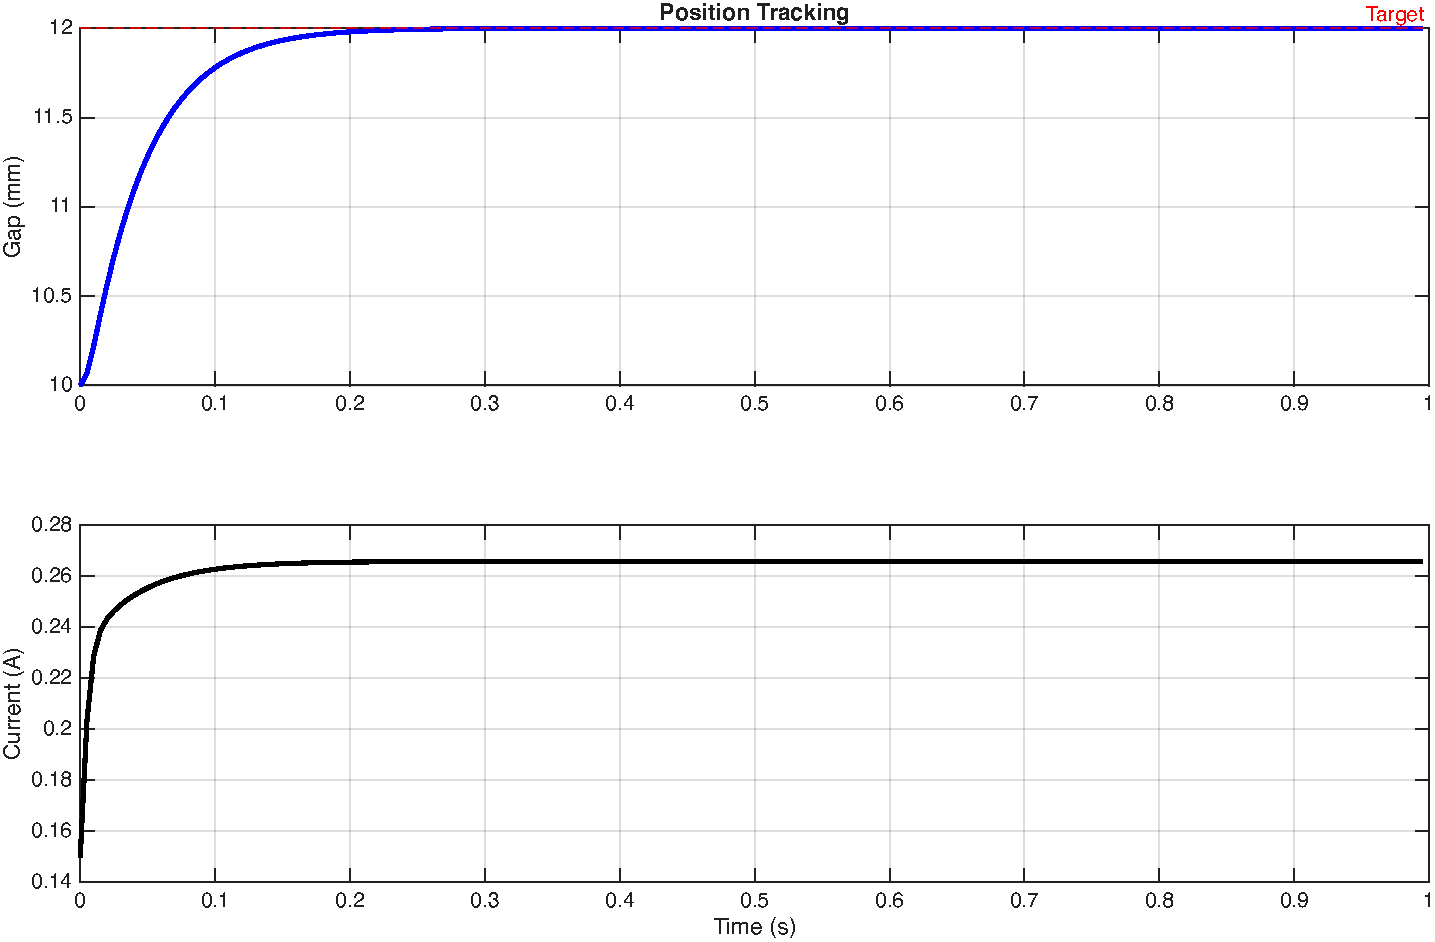
\includegraphics[width=0.7\linewidth]{Figures/Maglev.pdf}
		\captionof{figure}{Simulation results for the Magnetic Levitation setpoint tracking problem. 
			\textbf{Top:} The vertical gap (blue solid line) transitions smoothly from the initial equilibrium of 10 mm to the new target setpoint of 12 mm (red dashed line) with no overshoot. 
			\textbf{Bottom:} The control current settles at a new non-zero steady-state value ($\approx 0.26$ A). This illustrates the necessity of the feedforward term $u_g$: the current must remain non-zero to generate sufficient magnetic force to balance the weight of the ball at the new distance.}
		\label{fig:maglev}
	\end{center}
	
	
	
\end{examplebox}



\section{Chapter Summary}

This chapter has established the theoretical and numerical foundations of Optimal Control, marking the transition from system analysis to control synthesis. We introduced the LQR  as a specific instance of a broader optimisation framework.

By re-framing the classical recursive control problem as a batch QP, we laid the necessary groundwork for MPC. The key concepts covered in this chapter include:

\begin{itemize}
	\item \textbf{LQR as an Optimisation Problem:} We formulated the regulator problem as the minimisation of a quadratic cost function (penalising state deviations and control effort) subject to linear equality constraints imposed by the system dynamics.
	
	\item \textbf{The Batch Formulation:} We demonstrated how to stack decision variables into large, sparse vectors to cast the dynamic control problem into a standard static QP format ($\min \zeta^\top H \zeta$ s.t. $\mathcal{C}\zeta=d$). This perspective is critical for modern numerical solvers.
	
	\item \textbf{Equivalence of KKT and Riccati:} We proved that solving the KKT system of this QP via block back-substitution yields the classical Riccati recursion. This derivation confirmed that the optimal control law is a linear state feedback, $u_k = -K_k x_k$.
	
	\item \textbf{Infinite-Horizon Stability:} We showed that as the prediction horizon extends to infinity, the time-varying feedback gains converge to a constant steady-state value. This value can be computed directly via the Discrete Algebraic Riccati Equation (DARE), providing a static control law with guaranteed closed-loop stability.
	
	\item \textbf{Setpoint Tracking:} We extended the LQR framework from simple regulation (driving states to zero) to tracking non-zero setpoints. This requires an \textit{affine} control law combining a feedforward term (to maintain equilibrium) and a feedback term (to correct errors).
\end{itemize}

\section*{Exercises}
\begin{enumerate}
	\item Consider the discrete-time LTI system with
	\[
	A = \begin{bmatrix} 1 & 0.1 \\ 0 & 1 \end{bmatrix}, \quad B = \begin{bmatrix} 0.005 \\ 0.1 \end{bmatrix},
	\]
	and weighting matrices $Q = I_2$, $R = 1$.
	\begin{enumerate}
		\item Using the Riccati recursion with terminal cost $P_N = Q$, compute the feedback gain $K_{N-1}$ and the cost-to-go matrix $P_{N-1}$ by hand for a single backward step.
		\item Write down the resulting optimal control law $u_{N-1} = -K_{N-1}\,x_{N-1}$ and verify that the matrix $(R + B^\top P_N B)$ is invertible.
	\end{enumerate}

	\item For the same system as in Exercise~1, investigate the influence of the weighting matrices on the closed-loop behaviour.
	\begin{enumerate}
		\item Solve the DARE (using MATLAB's \texttt{dare} or an equivalent tool) for the following three design choices:
		\begin{itemize}
			\item $Q = I_2$, $R = 0.01$ \quad (cheap control),
			\item $Q = I_2$, $R = 1$ \quad (baseline),
			\item $Q = I_2$, $R = 100$ \quad (expensive control).
		\end{itemize}
		\item For each case, compute the steady-state gain $K$ and the eigenvalues of the closed-loop matrix $A_{cl} = A - BK$. Comment on how the magnitude of these eigenvalues changes as $R$ increases.
		\item Repeat the analysis by fixing $R = 1$ and varying $Q = \alpha I_2$ for $\alpha \in \{0.1,\; 1,\; 100\}$. Discuss the trade-off between fast state convergence and control effort.
	\end{enumerate}

	\item Consider the finite-horizon LQR cost function
	\[
	J = \frac{1}{2}\,x_N^\top P_N\,x_N + \sum_{k=0}^{N-1}\left(\frac{1}{2}\,x_k^\top Q\,x_k + \frac{1}{2}\,u_k^\top R\,u_k\right).
	\]
	Define the \emph{cost-to-go} at time step $k$ as
	\[
	J_k^*(x_k) = \frac{1}{2}\,x_k^\top P_k\,x_k.
	\]
	\begin{enumerate}
		\item Starting from the terminal condition $P_N = Q_N$, show by induction that $J_k^*(x_k) = \frac{1}{2}\,x_k^\top P_k\,x_k$ where $P_k$ satisfies the Riccati recursion
		\[
		P_k = Q + A^\top P_{k+1}(A - BK_k), \quad K_k = (R + B^\top P_{k+1} B)^{-1} B^\top P_{k+1} A.
		\]
		\item Explain why $P_k \succeq 0$ for all $k$ if $Q \succeq 0$, $R \succ 0$, and $P_N \succeq 0$.
	\end{enumerate}

	\item Let $P$ be the positive semi-definite solution of the DARE
	\[
	P = Q + A^\top P A - A^\top P B\,(R + B^\top P B)^{-1}\,B^\top P A.
	\]
	\begin{enumerate}
		\item Verify numerically (for the system in Exercise~1 with $Q = I_2$, $R = 1$) that $P$ is symmetric and positive definite.
		\item Substitute the computed $P$ back into the right-hand side of the DARE and confirm that both sides are equal (up to numerical precision).
		\item Define $K = (R + B^\top P B)^{-1} B^\top P A$ and compute the eigenvalues of $A_{cl} = A - BK$. Verify that all eigenvalues satisfy $|\lambda_i| < 1$, confirming closed-loop stability.
	\end{enumerate}

	\item Consider the open-loop unstable system
	\[
	A = \begin{bmatrix} 1.2 & 1 \\ 0 & 0.8 \end{bmatrix}, \quad B = \begin{bmatrix} 0 \\ 1 \end{bmatrix}.
	\]
	\begin{enumerate}
		\item Using classical pole placement, design a state-feedback gain $K_{\mathrm{pp}}$ that places the closed-loop eigenvalues of $(A - BK_{\mathrm{pp}})$ at $\lambda_1 = 0.3$ and $\lambda_2 = 0.5$.
		\item Design an infinite-horizon LQR controller for the same system with $Q = I_2$ and $R = 1$. Report the resulting gain $K_{\mathrm{lqr}}$ and the closed-loop eigenvalues.
		\item Compare the two designs: Which produces a larger control effort for the initial condition $x_0 = [1;\;0]$? Simulate both closed-loop systems for 30 time steps and discuss the differences in transient response and control magnitude. What advantages does the LQR design offer over ad-hoc pole placement?
	\end{enumerate}

	\item A student proposes to use the weighting matrices
	\[
	Q = \begin{bmatrix} 1 & 0 \\ 0 & -1 \end{bmatrix}, \quad R = 0.5
	\]
	in an LQR design.
	\begin{enumerate}
		\item Explain why this choice of $Q$ violates the convexity conditions required for a well-posed LQR problem.
		\item Provide a concrete example showing that the cost function $J = \sum_{k=0}^{N-1} \left(\frac{1}{2}\,x_k^\top Q\,x_k + \frac{1}{2}\,u_k^\top R\,u_k\right)$ can be made arbitrarily negative with this $Q$, and hence no finite minimum exists.
		\item Suggest a corrected $Q$ matrix that penalises only the first state variable (position) while leaving the second (velocity) unpenalised, and verify that it is positive semi-definite.
	\end{enumerate}
\end{enumerate}
